%============================================================================
\chapter{Building applications with XML templates}
%============================================================================

\section{Building a navigation}
%============================================================================

In OpenCms, the navigation concept is based on a representation of files and
folders of the VFS. To make a file or a folder appear 
in the navigation two properties must be added to the resource: 
The navigation position and the navigation text.

Whenever you create a new file or folder, a checkmark in the 
"New Page" / "New Folder" dialogue indicates whether this 
resource will be added to the navigation. You can then enter the 
navigation parameters position and text. Of course, those 
parameters can also be added, changed or deleted later.

If navigation entries should be grouped, then those elements have 
to be put in one folder. A folder can contain HTML files or 
further folders. An HTML file named index.html placed in a folder 
is being used as an overview for this folder. This means that if 
the folder name is, for example, {\dir /news/sport/}, clicking 
on this navigation entry will cause the file {\dir /news/sport/index.html} 
to be displayed. Because of this, the file does not need to be
included in the navigation.

If index.html does not exist, the navigation link will point to
the current folder. If you want the default file name to be changed
from index.html to another name (e.g. news.html), a property 
{\name NavIndex} containing the new file name has to be added to
the folder.

The OpenCms navigation properties can be easily read from a JSP 
using the OpenCms taglib or scriptlet API. 
How to do this is expained in the interactive part of the documentation.

In case you do not want to use JSP, you could also use the proprietary 
XML template mechanism to build navigation elements. 
{\em As of OpenCms 5.0, we recommend the use of JSP to build navigation elements.}

\section{Navigations with XML Templates}

The XML template mechanism brings along a set of methods in the class CmsXmlNav that
help you build a simple navigation. However, if a navigation with
extended functionality is needed, a new class extending CmsXmlNav
has to be written for with XML Templates (this is not required if you use JSP)

To display the navigation, an element {\name nav} must be defined
in the frametemplate of the files. In the element definition of
this element, the class CmsXmlNav and a template file {\name
navigation} must be defined. The template of this element is used
to define the required HTML-code to build the navigation. Example:
First the frametemplate:

%\input{examples/templateMechanism/navigation/frametemplateNav}
\begin{verbatim}
<?xml version="1.0" encoding="ISO-8859-1"?> 
<XMLTEMPLATE> 
<TEMPLATE><![CDATA[
    <HTML>
    <HEAD>
        <TITLE>]]><method name="getTitle"/><![CDATA[</TITLE>
    </HEAD>
    <BODY>
    <TABLE border width="100\%" height="100\%">
        <TR height="30\%">
        <TH colspan=2 width="100\%" align="center">
            The Head section
        </TH>
        </TR>
        <TR height="70\%">
        <TD width="20\%" align="center" valign="top">
            ]]><element name="nav"/><![CDATA[
        </TD>
        <TD width="80\%" align="center">
            ]]><element name="contenttemplate"/><![CDATA[
        </TD>
    </TR>
    </TABLE>
    </BODY>
    </HTML>]]>
</TEMPLATE>

<ELEMENTDEF name="nav">
    <CLASS>com.opencms.defaults.CmsXmlNav</CLASS>
    <TEMPLATE>/system/modules/org.opencms.default/elements/navigation</TEMPLATE>
</ELEMENTDEF>

</XMLTEMPLATE>
\end{verbatim}
\index{ELEMENTDEF}
\index{element}
\index{getTitle}

Now the definition of the navigation element in 
{\dir /system/modules/org.opencms.default/elements/}

%\input{examples/templateMechanism/navigation/navigation}
\begin{verbatim}
<?xml version="1.0" encoding="ISO-8859-1"?> 
<XMLTEMPLATE>

<naventry>
    <![CDATA[
    <tr>
     <td>
      <a href="]]><process>navlink</process><![CDATA[">
             ]]><process>navtext</process><![CDATA[
      </a>
     </td>
    </tr>
    ]]>
</naventry>

<navcurrent>
    <![CDATA[
    <tr>
     <td>
       ]]><process>navtext</process><![CDATA[
     </td>
    </tr>
    ]]>
</navcurrent>

<TEMPLATE>
    <![CDATA[
    <TABLE border width="100\%" height="100\%">
      ]]><method name="getNavCurrent"/><![CDATA[
    </TABLE>
    ]]>
</TEMPLATE>
</XMLTEMPLATE>
\end{verbatim}
\index{ELEMENTDEF}
\index{element}
\index{getNavCurrent}

Several data block definitions and one method are used in this 
example. The definition of the {\name naventry} data block is 
compulsory, otherwise no element of navigation would be shown. 
It is used to generate navigation entries. The {\name navcurrent} 
data block is used to show the current position in the navigation. 
It can be used to highlight the current navigation entry, e.g.
using a different font color or style. \\
The method {\name getNavCurrent} is a method defined in class 
CmsXmlNav and returns the navigation of the current folder. \\

The following methods defined in CmsXmlNav class can be used 
to build different types of navigation. Here is the definition 
of methods, tools and data blocks defined in the CmsXmlNav 
class: \\

Data blocks that have to be defined in the templates managed 
by CmsXmlNav: \\

- navtext \index{navtext} \\
- navlink \index{navlink} \\
- naventry \index{naventry} \\
- navcurrent \index{navcurrent} \\
- navstart \index{navstart} \\
- navend \index{navend} \\

Additional data blocks that can be of use in a navigation structure: \\

- navlevel \index{navlevel} \\
- navcount \index{navcount} \\

Methods that are defined in CmsXmlNav: \\

- getNavCurrent \index{getNavCurrent} \\
- getNavFold \index{getNavFold} \\
- getNavTree \index{getNavTree} \\
- getNavParent \index{getNavParent} \\
- getNavRoot \index{getNavRoot} \\


Additional methods that could be helpful in templates: \\

- getFolderCurrent \index{getFolderCurrent} \\
- getFolderParent \index{getFolderParent} \\
- getFolderRoot \index{getFolderRoot} \\
- getPropertyCurrent \index{getPropertyCurrent} \\
- getPropertyParent \index{getPropertyParent} \\
- getPropertyRoot \index{getPropertyRoot} \\
- getPropertyUri \index{getPropertyUri} \\
\subsubsection{Definition of data blocks:}
\subsubsection{- navtext:} \index{navtext}
  This data block is used to display the navigation text. 
The navigation text is defined in the {\name NavText} property 
of the corresponding file or folder. \\

\subsubsection{- navlink:} \index{navlink}
%============================================================================

  This data block shows the path of the corresponding 
navigation entry.\\

\subsubsection{- naventry:} \index{}
%============================================================================

  The definition of this data block is compulsory, because 
this data block defines the layout of a navigation entry. 
For each navigation entry this data block is used. Example: \\

  \begin{xml}
  <naventry> \\
  <![CDATA[ \\
  <tr> \\
  \xtaba <td> \\
  \xtabb   <a href="]]><process>navlink</process><![CDATA[ class="nav" target="\_blank"> \\
  \xtabc      ]]><process>navtext</process><![CDATA[ \\
  \xtabb   </a> \\
  \xtaba </td> \\
  </tr> \\
  ]]> \\
  </naventry> \\
  \end{xml}

\subsubsection{- navcurrent:} \index{navcurrent}
%============================================================================

  With the definition of this data block, the layout of the current 
navigation position is set. If this data block is not defined, the 
{\tag <naventry>} data block is used. Example: \\

  \begin{xml}
  <navcurrent> \\
  <![CDATA[ \\
  <tr> \\
  \xtaba <td> \\
  \xtabb   <font color="red">]]><process>navtext</process><![CDATA[</font> \\
  \xtaba </td> \\
  </tr> \\
  ]]> \\
  </navcurrent> \\
  \end{xml}

\subsubsection{- navstart and navend:} \index{navstart} \index{navend}
%============================================================================

  These data blocks are used in nested navigation system, so if the methods 
{\name getNavFold} or {\name getNavTree} are used then these data blocks 
can be used to format the navigation. These methods work recursively and 
after each call these data blocks are used to format the navigation entries. 
For example, a definition of the data block {\tag <navstart>} 
as a {\tag <ul>} tag and the {\tag <navend>} data block as a {\tag </ul>} 
tag creates a nested {\tag <ul>} ... {\tag </ul>} list. Example: \\

  \begin{xml}
  <navstart><![CDATA[<ul>]]></navstart> \\
  <naventry><![CDATA[ \\
    \xtaba <li> \\
    \xtaba <a href="]]><process>navlink</process><![CDATA["> \\
    \xtabb ]]><process>navtext</process><![CDATA[ \\
    \xtaba </a>]]> \\
  </naventry> \\
  <navcurrent><![CDATA[<li>]]><process>navtext</process></navcurrent> \\
  <navend><![CDATA[</ul>]]></navend> \\
  \end{xml}

  If the {\tag <navstart>} and {\tag <navend>} are not defined then they are ignored. \\

\subsubsection{- navlevel:} \index{navlevel}
%============================================================================

  This data block contains the depth of the navigation entry. This data 
block could be used in a nested navigation system, e.g. the definition of a 
group of style sheets depending on the depth of navigation. Example: \\

  \begin{xml}
  <navstart><![CDATA[<ul>]]></navstart> \\
  <naventry><![CDATA[ \\
  \xtaba <li class="nav\_]]><process>navlevel</process><![CDATA["> \\
  \xtaba <a class="nav\_]]><process>navlevel</process><![CDATA[" \\
  \xtaba href="]]><process>navlink</process><![CDATA["> \\
  \xtabb ]]><process>navtext</process><![CDATA[ \\
  \xtaba </a>]]> \\
  </naventry> \\
  <navcurrent><![CDATA[ \\
      <li class="nav\_]]><process>navlevel</process><![CDATA["> \\
      ]]><process>navtext</process> \\
  </navcurrent>\\
  <navend><![CDATA[</ul>]]></navend>\\
  \end{xml}

  With <navlevel>, the depth of the navigation entry is determined. 
With a corresponding definition of the style sheet in a .css 
file (e.g. nav\_1{....},nav\_2{....},nav\_3{....}, ....), each level 
of the navigation can be formatted in different way. \\

  Should the level number be given as a parameter in a method, then 
the real depth will be calculated from the difference of depth 
between the current folder and the given depth in the method. \\

\subsubsection{- navcount:} \index{navcount}
%============================================================================

  An additional data block that returns the number of navigation 
entries in the navigation. \\
\subsubsection{Definition of Methods:}
\subsubsection{- getNavCurrent:} \index{getNavCurrent}
  This method gets the navigation of the current folder, using the 
{\name naventry} and {\name navcurrent} data blocks.\\

\subsubsection{- getNavFold:} \index{getNavFold}
%============================================================================

  This method gets the navigation of a specified folder. If an entry 
is clicked, then the navigation of that entry will be added to the 
current navigation. Because of folding functionality this method 
is called getNavFold. \\
  This method uses the {\tag <naventry>}, {\tag <navcurrent>}, 
{\tag <navstart>} and {\tag <navend>} data blocks. \\

  A level parameter can be set as follows: \\
  {\tag <method name="getNavFold/>} \\
  {\tag <method name="getNavFold>level</method>} \\

  The level parameter defines the starting folder of navigation from 
which the navigation will be constructed. For example, if the current 
folder is {\dir /news/sport/foot\-ball/li\-ga/first/} and the method 
definition is {\tag <method name="getNavFold>2</method>}, then the 
starting folder for the navigation will be {\dir /sport/} and all 
elements starting from {\tag /sport/} will be displayed.\\

  If no level parameter is defined, the starting point is set to the 
root folder. \\

\subsubsection{- getNavTree:} \index{getNavtree}
%============================================================================

  This method gets the navigation starting from a folder and shows 
the wholer navigation tree recursively. Therefore, this method is 
called {\name getNavTree}. \\

  Level and depth parameter can be set as follows: \\
  {\tag <method name="getNavTree/>} \\
  {\tag <method name="getNavTree>level</method>} \\
  {\tag <method name="getNavTree>level,depth</method>} \\

  The level parameter defines the starting folder from which the 
navigation will be constructed. For example, if the current folder is 
{\dir /news/sport/foot\-ball/li\-ga/first/} and the method definition is 
{\tag <method name="getNavTree>2</method>} then the starting folder for the 
navigation will be {\dir /sport/} and all elements starting from 
{\dir /sport/} folder will be displayed. \\

  If no level parameter is defined, the starting point is set to the 
root folder. \\

  The depth parameter defines how many levels of folders will be displayed 
in the navigation tree. For example, if the current folder is 
{\dir /news/sport/football/liga/first/} and the method definition is 
{\tag <method name="getNavTree>1,3</method>} then the starting folder for 
the navigation will be {\dir /news/} and all elements from {\dir /news/} 
to {\dir /news/sport/football/} will be displayed. \\

\subsubsection{- getNavParent:} \index{getNavParent}
%============================================================================

  This method gets the navigation from the parent folder(s), depending on the 
given depth parameter. For example, if the current Folder is 
{\dir /news/sport/football/liga/first/} and the method definition is 
{\tag <method name="getNavParent>2</method>} then the navigation of the folder 
{\dir /news/sport/football/} will be displayed (two levels up). If no depth 
parameter is given, the navigation of the current folder will be displayed. 
If the number given as depth parameter exceeds the sum of possible folders, 
the root folder will be chosen. \\


\subsubsection{- getNavRoot:} \index{getNavRoot}
%============================================================================

  This method gets a navigation tree starting from the root folder, depending 
on the given parameter. If, for example, the current folder is 
{\dir /news/sport/football/liga/first/} and the method definition is 
{\tag <method name="getNavRoot>2</method>}, then the navigation of 
{\dir /news/sport/} will be displayed (second level starting from root). 
If no depth parameter is given, the current folder's navigation is chosen. 
If the number given as depth parameter is too high, the current folder will be chosen. \\

\subsubsection{- getFolderCurrent:} \index{getFolderCurrent}
%============================================================================

This method gets the current folder. It provides the same functionality as {\name getPathUri} in class CmsXmlTemplate used in many templates. \\

\subsubsection{- getFolderParent:} \index{getFolderParent}
%============================================================================

 This method gets the parent folder, depending on the depth parameter given. For example, 
if the current folder is {\dir /news/sport/football/liga/first/} and the method 
definition is {\tag <me\-thod name="get\-Folder\-Parent>2\-</me\-thod>}, the folder 
returned by this method will be {\dir /news/sport/football/}. If no 
parameter is given, the current folder will be returned. If the number given as 
depth parameter is too high, the root folder will be returned. \\

\subsubsection{- getFolderRoot:} \index{getFolderRoot}
%============================================================================

  This method gets a specific folder underneath the root folder, depending on the depth 
parameter given. If, for example, the current folder is {\dir /news/sport/football/liga/first/} 
and the method definition is {\tag <method name="getFolderRoot>2</method>}, then the 
folder {\dir /news/sport/} will be displayed (second level starting from root). If 
no depth parameter is given, the root folder will be returned. If the number given 
as depth parameter is too high, the current folder will be returned. \\

\subsubsection{- getPropertyCurrent:} \index{getPropertyCurrent}
%============================================================================

  This method gets a property of the current folder. This method is used as follows:\\
{\tag <method name="getProperyCurrent">property</method>} \\
where property is the name of the property to be displayed. If there is no such property name, 
nothing is returned. \\

\subsubsection{- getPropertyParent:} \index{getPropertyParent}
%============================================================================

 This method gets the property of a parent folder, depending on the parameters given. This 
method is used as follows:\\
{\tag <method name="getPropertyParent">level,property</method>} \\
where {\name property} is the name of the property to be read. If there is no such property name, 
nothing is returned. \\
{\name level} is the number of folders to go up. If, for example, the current folder is 
{\dir /news/sport/foot\-ball/li\-ga/first/} and the method definition is \\
{\tag <me\-thod name="get\-Property\-Parent">2,NavPic</me\-thod>}, the value of the 
{\name NavPic} property of {\dir /news/sport/football/} would be returned by 
this method. If the number given as level parameter is too high, the same property of 
the root folder is read. \\


\subsubsection{- getPropertyRoot:} \index{getPropertyRoot}
%============================================================================

  This method gets the property of a specified folder underneath the root folder, depending 
on the level parameter given. This method is as follows:\\
{\tag <method name="getPropertyRoot">level,property</method>} \\
where {\name property} is the name of the property to be read. If there is no such property 
name, nothing is returned.\\
{\name level} specifies the number of folders to go down from the root folder. If, for 
example, the current folder is {\dir /news/sport/foot\-ball/li\-ga/first/} and the method 
definition is {\tag <method name="get\-Property\-Root">2,NavPic</me\-thod>}, the value of 
the property {\name NavPic} of {\dir /news/sport/} will be returned by this 
method. If the number given as level parameter is too high, the same property of the 
current folder is returned. \\


\subsubsection{- getPropertyUri:} \index{getPropertyUri}
%============================================================================

  This method returns the specified property of the current uri. This method is used as follows:\\
{\tag <method name="getProperyUri">property</method>} \\
where {\name property} is the name of the property to be read. If there is no such property 
name, nothing is returned. \\


It is very common to use an image instead of Text in navigation. Therefore, here is 
an example that uses images instead of text: \\

\begin{xml}
<?xml version="1.0" encoding="ISO-8859-1"?> \\
<XMLTEMPLATE> \\

<naventry> \\
<![CDATA[ \\
<tr> \\
\xtaba <td> \\
\xtabb   <a href="]]><process>navlink</process><![CDATA[" \\
\xtabc   onmouseover="JavaScript:document.image\_ \\
\xtabc   ]]><process>count</process><![CDATA[.value= \\
\xtabc   '/pics/templates/]]><process>navtext</process> \\
\xtabc   <![CDATA[\_light.gif'" \\
\xtabc   onmouseout="JavaScript:document.image\_]]> \\
\xtabc   <process>count</process><![CDATA[.value= \\
\xtabc   '/pics/templates/]]><process>navtext</process><![CDATA[.gif'"> \\
\xtabc   <img name="image\_]]><process>count</process><![CDATA[" \\
\xtabc   src="/pics/templates/ \\
\xtabc   ]]><process>navtext</process><![CDATA[.gif"> \\
\xtabb   </a> \\
\xtaba </td> \\
</tr> \\
]]> \\
</naventry> \\

<navcurrent> \\
<![CDATA[ \\
<tr> \\
\xtaba  <td> \\
\xtabb    <img src="/pics/templates/]]><process>navtext</process><![CDATA[.gif"> \\
\xtaba  </td> \\
</tr> \\
]]> \\
</navcurrent> \\

<TEMPLATE> \\
<![CDATA[ \\
<TABLE border width="100\%" height="100\%"> \\
\xtaba  ]]><method name="getNavCurrent"/><![CDATA[ \\
</TABLE> \\
]]> \\
</TEMPLATE> \\

</XMLTEMPLATE> \\
\end{xml}


To build a navigation using images instead of text, an image name must be written in the property
{\name NavText}. To get mouse over and mouse out effects, another picture with the same name but 
with a suffix is needed so that javascript can replace it. In the example above, the 
image name is built with the count data block (so image\_1, image\_2,.... 
would be generated). Then, the picture for the mouse over effect is included with the count
data block and the suffix {\name \_light}. So if the picture 
name is {\name nav.gif}, then the mouse over picture would be nav\_light.gif. \\

\section{Frames}
%============================================================================

\subsection{Frames with XML templates}
%============================================================================

 \index{frames}
The usage of frames is possible with proprietary XML templates. One big difference
to the usage of frames in standard HTML is that in with XML templates,
the frameset and all frames are defined together in one file.  In this part, we will
create a simple page with two frames to show the basic structure.
The frameset and the inserted parts (templates) are defined in the
frametemplate. The complete code for a frametemplate with 2 frames
is shown here:
\begin{xml}
<?xml version="1.0" encoding="ISO-8859-1"?>\\
<XMLTEMPLATE>\\

<TEMPLATE><![CDATA[\\
<!DOCTYPE HTML PUBLIC "-//W3C//DTD HTML 4.0 Transitional//EN">\\
<HTML>\\
  <HEAD><TITLE>Seite mit Frames</TITLE></HEAD>\\
  <FRAMESET ROWS="100,*">\\
\xtaba     <FRAME NAME="frame\_head" src="]]>\\
\xtabb <METHOD name="getUri"/>\\
\xtabb            <METHOD name="getFrameQueryString">temp\_head</METHOD>\\
\xtabb            <![CDATA[">\\
\xtaba     <FRAME NAME="frame\_body" src="]]>\\
\xtabb            <METHOD name="getUri"/>\\
\xtabb            <METHOD name="getFrameQueryString">temp\_body</METHOD>\\
\xtabb            <![CDATA[">\\
  </FRAMESET>\\
</HTML>]]>\\
</TEMPLATE>\\
\index{getFrameQueryString}
<TEMPLATE name="temp\_head"><![CDATA[\\
\xtaba <!DOCTYPE HTML PUBLIC "-//W3C//DTD HTML 4.0 Transitional//EN">\\
\xtaba <HTML>\\
\xtaba   <HEAD><TITLE>Seite mit Frames</TITLE></HEAD>\\
\xtaba   <BODY>\\
\xtabb             <P ALIGN="center">\\
\xtabb       ]]><ELEMENT name="nav\_head"/><![CDATA[\\
\xtabb     </P>\\
\xtaba   </BODY>\\
\xtaba </HTML>]]>\\
</TEMPLATE>\\

<TEMPLATE name="temp\_body"><![CDATA[\\
\xtaba <!DOCTYPE HTML PUBLIC "-//W3C//DTD HTML 4.0 Transitional//EN">\\
\xtaba <HTML>\\
\xtaba   <HEAD><TITLE>Seite mit Frames</TITLE></HEAD>\\
\xtaba   <BODY>\\
\xtabb     <P ALIGN="center">\\
\xtabb       ]]><ELEMENT name="contenttemplate"/><![CDATA[\\
\xtabb     </P>\\
\xtaba   </BODY>\\
\xtaba </HTML>]]>\\
</TEMPLATE>\\

<ELEMENTDEF name="nav\_head">\\
\xtaba <CLASS>com.opencms.defaults.CmsXmlNav</CLASS>\\
\xtaba <TEMPLATE>/system/modules/org.opencms.default/elements/nav\_head</TEMPLATE> \\
</ELEMENTDEF>\\

</XMLTEMPLATE>\\
\end{xml}


The frameset is here defined within the default template (the one
without a name) with the normal {\tag <FRAMESET>} tag. The content
of the frames is defined in the other templates (temp\_head and temp\_body).
The link to the frames is created by using the two XML template methods
{\meth getUri()} and {\meth getFrameQueryString()}. The method
{\meth getUri()} returns the URI of the currently requested page
and the method {\meth getFrameQueryString()} returns the original query string
of the request together with an additional parameter {\name cmsframe}
which determines what template is to be used. The value of the
cmsframe parameter is passed to the {\meth getFrameQueryString()} method
as the tagcontent of the {\tag <METHOD>} tag. For example the 
line:

\begin{xml}
<METHOD name="getFrameQueryString">temp\_head</METHOD>\\
\end{xml}

results in this text:
\begin{xml}
?cmsframe=temp\_head
\end{xml}

It would be possible to simply add the parameter by hand:

\begin{xml}
<![CDATA[?cmsframe=temp\_head
\end{xml}

This would cause problems if further parameters are appended to the
URL because they would not be included in this string. The method {\meth
getFrameQueryString()} solves this problem and handles further
parameters. Thus it is recommended to use the method always.
\index{cmsframe} 

Our frametemplate includes two elements, one for the navigation
(nav\_head) and one content element. Of course, there has to be an
elementdefinition for the navigation element at the end of the
XML-file.  The navigation template for this example looks like
this:

\begin{xml}
<?xml version="1.0" encoding="ISO-8859-1"?>\\
<XMLTEMPLATE>\\

<NAVENTRY><![CDATA[\\
\xtaba   <A HREF="]]>\\
\xtaba   <PROCESS>navlink</PROCESS>\\
\xtaba     <METHOD name="getFrameQueryString">temp\_body</METHOD>\\
\xtaba     <![CDATA[" ]]>\\
\xtaba     <METHOD name="getFrameTarget">frame\_body</METHOD>\\
\xtaba     <![CDATA[>]]>\\
\xtaba   <PROCESS>navtext</PROCESS><![CDATA[\\
\xtaba   </A>]]>\\
</NAVENTRY>\\

<TEMPLATE>\\
\xtaba   <![CDATA[<TABLE BORDER=1 CELLPADDING=2 CELLSPACING=0><TR><TD>]]>\\
\xtaba   <METHOD name="getNavRoot">1</METHOD>\\
\xtaba   <![CDATA[</TD></TR></TABLE>]]>\\
</TEMPLATE>\\

</XMLTEMPLATE>\\
\end{xml}
\index{getNavRoot}
\index{getFrameTarget}

A reference to a page that should be displayed in another frame in standard HTML looks like
this:

{\tag <a href="aName.htm" target="aFrame">aNavText</a>}

The parameter {\name aFrame} determines the frame in which the source should be displayed,
and the parameter {\name aName.htm} determines the source that should be inserted.
Here the parameter {\name aName.htm} has to be expanded by a parameter that defines what template has
to be selected to insert. This is again done by the templateselector, and the parameter
{\name cmsframe} is again inserted by the method {\meth getFrameQueryString()} to allow further
parameters.

\begin{xml}
<A HREF="]]>\\
  <PROCESS>navlink</PROCESS>\\
    <METHOD name="getFrameQueryString">temp\_body</METHOD>\\
    <![CDATA[" ]]>\\
    <METHOD name="getFrameTarget">frame\_body</METHOD>\\
    <![CDATA[>]]>\\
  <PROCESS>navtext</PROCESS><![CDATA[\\
</A>]]>\\
\end{xml}


The parameter {\name target} is here inserted by the method {\meth getFrameTarget()}. 
Of course, the parameter could be simply added by inserting
{\tag target="frame\_body"}, but you will see in the next paragraph why the usage of the method
has advantages.
To understand the difference, the above code block is now shown without the usage of
methods:
\begin{xml}
<A HREF="]]>\\
  <PROCESS>navlink</PROCESS>\\
    <!CDATA[?cmsframe="temp\_body" TARGET="frame\_body">]]>\\
  <PROCESS>navtext</PROCESS><![CDATA[\\
</A>]]>\\
\end{xml}


Maybe this helps to understand which text is inserted by the methods. But again, it is allways
recommended to make usage of these methods, to write templates that can be easily reused and
provide full functionality.

Pages which use our frame structure can now easily be created. 
You only have to choose the above mastertemplate. 
The output for three inserted pages could for example look like
figure~\ref{frames1}.

\begin{figure}[hbt]
\begin{center}
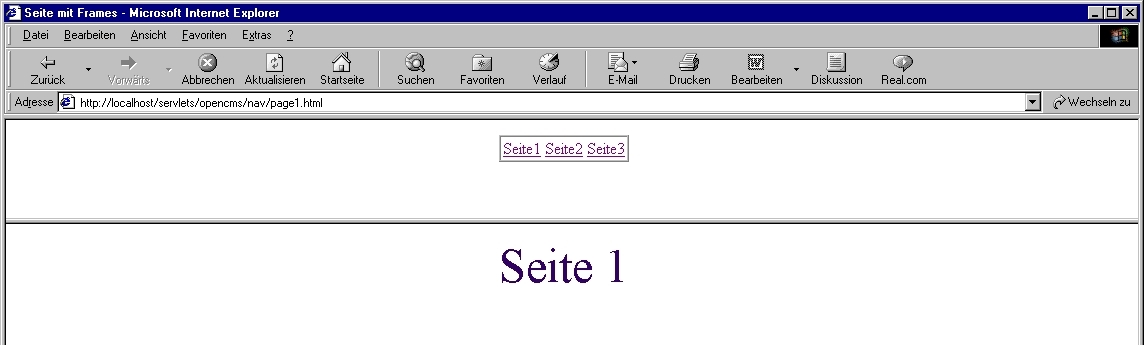
\includegraphics[width=\sgw]
                   {pics/templateMech/frames_kurz}
\caption[A page with frames]
           {A page with frames}
\label{frames1}
\end{center}
\end{figure}

\subsection{Frames- and noframes versions of a website with XML templates}

Often a website has to be build in two versions: one with frames,
and one without frames. This way users with older browsers are
able to visit the site as well. These two versions can be achieved
with one frametemplate. All you have to do is to extend
the frametemplate by one further template. This template should
be named {\name plain}. It defines the layout for the site without
frames. One implementation of the {\name plain}-template is shown now:

\begin{xml}
<?xml version="1.0" encoding="ISO-8859-1"?>\\
...\\
<TEMPLATE name="plain"><![CDATA[\\
<HTML> \\
<HEAD>\\
\xtaba <TITLE>]]><method name="getTitle"/><![CDATA[</TITLE>\\
</HEAD>\\
<BODY>\\
\xtaba <TABLE border width="100\%" height="100\%">\\
\xtaba   <TR height="30\%">\\
\xtabb             <TD align="center">]]> \\
\xtabb              <element name="nav\_head"/> <![CDATA[</TD>\\
\xtaba   </TR>\\
\xtaba   <TR height="70\%">\\
\xtabb             <TD align="center">]]>\\
\xtabb              <element name="body"/> <![CDATA[</TD>\\
\xtaba   </TR>\\
\xtaba </TABLE>\\
</BODY>\\
</HTML>]]>\\
</TEMPLATE>\\

<ELEMENTDEF name="nav\_head">\\
...\\
</XMLTEMPLATE>\\
\end{xml}

This template inserts exactly the same subtemplates as the one that uses frames. Even the
template for the navigation is the same. They are only set inside a table instead of frames.
Now it becomes useful that we implemented the navigation with the {\meth getFrameTarget()} 
method.
The navigation would not work with a table, if the parameter {\tag target=...} had
simply be added. The {\meth getFrameTarget()} method distinguishes between the frames and
the noframes version and drops the parameter {\name target} if necessary. 
If you implemented the templates like this, a simple call to the URL of a page that 
uses this mastertemplate would start the frames version, which is defined in
the default template. 
You can choose the noframes version by adding the parameter {\name ?cmsframe=plain}
to the URL. The output would then look like figure~\ref{noFrames}.

\begin{figure}[hbt]
\begin{center}
\includegraphics[width=\sgw]
                   {pics/templateMech/frames_2}
\caption[A version without frames]
           {A version without frames}
\label{noFrames}
\end{center}
\end{figure}

\section{The CmsObject Class (accessing system resources)}
%============================================================================

There is a a programming interface that provides access to the
system and all of its resources. The majority of the interface is part
of the {\name CmsObject} that provides methods to access system resources.
These resources can be for example files, user data or session-related
data. The {\name CmsObject} enables these resources to be manipulated (i.e.
deleted, renamed, moved) and properties of these resources to be
requested. Since all of the operations performed by the {\name CmsObject} are
executed by the user that is currently accessing the system, access to
the system resources is limited by that user's access permissions.
Using the API (Application Programming Interface) provided by the
{\name CmsObject} enables you to create customized classes that perform various
kinds of operations.
The next sections will explain how common tasks can be accomplished by
using the {\name CmsObject} and its API. Only a short collection of the
available {\name CmsObject} methods is used in the following examples. The
complete API can be found as JavaDoc in the appendix.

\subsection{Accessing user data}
%============================================================================

The OpenCms user management can be accessed via the API to read or
write the users maintained by the system. The following example will
read all users of the system and will display them in a simple HTML
table. 

All of the following examples that use the CmsObject generate highly dynamic
content, therefore it is necessary to override the {\meth getCacheDirectives()} 
\index{getCacheDirectives()}
method in the template classes of this examples and set the internal caching
to false in the returned {\class CmsCacheDirectives} 
\index{CmsCacheDirectives}
object. See section \ref{element cache} (page \pageref{element cache})
for details about the element caching.

First, all of the users have to be read from the OpenCms system. This
is done in the {\meth getContent} method of the template class, and is achieved
by using the following {\meth CmsObject} method:\\


{\meth // get all users\\

Vector users=cms.getUsers();}\\

This returns a vector of {\name CmsUser} objects, each of which contains the
data of a single OpenCms user. The individual {\name CmsUsers} are extracted from the
vector and their login, first and last names as well as their e-mail
address are read. See the appendix for a complete overview of the
{\name CmsUser} object methods.

The HTML table is built in a similar way to the table in the animal
list example (see page \pageref{animal list example}): 
a row of the table is defined as a data block in the
template file, that contains several {\tag <process>} tags that must be
filled by the Java class. The rows are generated for each {\name CmsUser}
entry in order to create a complete list of users.\\

The complete getContent Method of this example looks like this:\\

\begin{java}
public byte[] getContent(CmsObject cms, String templateFile, String\\
\jtaba   elementName, Hashtable parameters, String\\
\jtaba   templateSelector) throws CmsException \{\\

CmsXmlTemplateFile template = getOwnTemplateFile(cms, templateFile,\\
\jtaba   elementName, parameters,\\
\jtaba   templateSelector);\\

\jtabc        // get all users\\
\jtabc        Vector users=cms.getUsers();\\

\jtabc        String list="";\\

\jtabc        // browse through all users\\
\jtabc        for (int i=0;i<users.size();i++) \{\\
\jtabd                //get a single user\\
\jtabd                CmsUser user=(CmsUser)users.elementAt(i);\\
\jtabd                template.setData("name",user.getName());\\
\jtabd                template.setData("firstname",user.getFirstname());\\
\jtabd                template.setData("lastname",user.getLastname());\\
\jtabd                template.setData("email",user.getEmail());\\
\jtabd                String row=template.getProcessedDataValue("row");\\
\jtabd                list+=row;\\
\jtabc        \}\\

\jtabc        template.setData("list", list);\\

\jtabc        return startProcessing(cms, template, elementName, parameters,\\
\jtabc            templateSelector);\\
\}\\
\end{java}

This example can easily be extended to read additional user information
that is stored in the OpenCms database by adding the access methods to
the other data fields.

\subsubsection{Reading Resource Properties}
Resources in the OpenCms VFS can have additional properties. By default,
these properties are used to store the resource title, but they could
also be used to store additional information that is used by the
template class. For example this could be the name of an image that
must be different for all pages that use a special template, or
information on where the Java class can find additional data. Another
typical use for the resource properties is to store information that is
necessary to build a dynamic navigation.\\

The following example shows how to read all of a resource's properties
and display them in an HTML table.\\

First, the name of the current resource - the URI - must be read. This
is done by using the {\name CmsRequestContext}. There, all of the data that
belongs to the actual request, i.e. User, Project, HttpRequest,
HttpResponse and Session are stored:\\

\begin{java}
// get the uri of the requested file\\
 String uri=cms.getRequestContext().getUri();\\
\end{java}

The getUri method returns the complete path of the current resource in
the VFS. See the appendix for a complete overview of the
{\name CmsRequestContext's} methods.

In the next step all of the {\name resource's} properties are read. This is
done using a CmsObject method that returns a hash table that contains
the {\name properties'} names and values:

\begin{java} 
// get all propereties of this resource\\
 Hashtable prop=cms.readAllProperties(uri);\\
\end{java}

Now that all of the data is fetched from the system, the output must be
generated. This is done in almost the exact same way that it was in the
previous example:

\begin{java}
public byte[] getContent(CmsObject cms, String templateFile, String\\
\jtaba   elementName, Hashtable parameters, String\\
\jtaba   templateSelector) throws CmsException \{\\

CmsXmlTemplateFile template = getOwnTemplateFile(cms, templateFile,\\
\jtabe                              elementName, parameters,\\
\jtaba   templateSelector);\\

\jtaba        // get the uri of the requested file\\
\jtaba        String uri=cms.getRequestContext().getUri();\\

\jtaba        // get all propereties of this resource\\
\jtaba        Hashtable prop=cms.readAllProperties(uri);\\

\jtaba        Enumeration en=prop.keys();\\

\jtaba        String list="";\\

\jtaba        while (en.hasMoreElements()) \{\\
\jtabc            String key=(String) en.nextElement();\\
\jtabc            String value=(String)prop.get(key);\\

\jtabc            template.setData("property",key);\\
\jtabc            template.setData("value",value);\\
\jtabb         String row=template.getProcessedDataValue("row");\\
\jtabc            list+=row;\\

\jtaba        \}\\


\jtaba        template.setData("filename",uri);\\
\jtaba        template.setData("list",list);\\

\jtaba        return startProcessing(cms, template, elementName, parameters,templateSelector);\\
\}\\
\end{java}

As an alternative, a single resource property can be read with the
following line of code:

{\code String value=cms.readProperty(uri,key);}

This will either return the value of the property with the name
"propertyname," or null if this property does not exist.

\subsection{Resource access}
%============================================================================

A typical task for a template programmer is to read the resources that
are stored in the VFS. The {\name CmsObject} contains several methods that
enable a programmer to read either a single resource - this could be a
file or a folder - or a complete vector of subresources - the files or
subfolders of a specified folder.

The next example will create a list of all of the folders that are
stored in the VFS, that contains their complete path and
title (if existing). It consists of a simple {\meth getContent()} method that calls a
recursive {\meth getFolders()} method that produces the HTML output of folder
list of a given root folder. The manner in which the HTML output is
created is similar to that shown in the previous examples.

\begin{java}
public class CmsExample21 extends CmsXmlTemplate\\ 
public byte[] getContent(CmsObject cms, String templateFile, String\\
elementName, Hashtable parameters, String templateSelector)\\
throws CmsException\\ 
CmsXmlTemplateFile template = getOwnTemplateFile(cms, templateFile,\\
elementName, parameters, templateSelector);\\
\jtabc        String list=getFolders(cms,template,"/");\\
\jtabc        template.setData("filename","/");\\
\jtabc        template.setData("list",list);\\

return startProcessing(cms, template, elementName, parameters,\\
templateSelector);\\
\}\\
\end{java}

The core functions of this template class are located in the {\meth getFolders()}
method:

\begin{java}
private String getFolders(CmsObject cms, CmsXmlTemplateFile template,String root)\\
\jtabc        throws CmsException\{\\
\jtabd           String list="";\\
// get all subfolders of the root folder Vector folders=cms.\\
\index{getSubFolders}
getSubFolders(root);\\
\jtabd           // build the list of folders\\
\jtabd           for (int i=0;i<folders.size();i++) \{\\
\jtabd           CmsFolder folder=(CmsFolder)folders.elementAt(i);\\
\jtabd           String foldername=folder.getAbsolutePath();\\
String      foldertitle=cms.readProperty(foldername,"Title");\\
template.setData("resource",foldername); template.setData("name",foldertitle);\\
\jtabd           String row=template.getProcessedDataValue("row");\\
\jtabd           list+=row;\\
\jtabd           list+=getFolders(cms,template,foldername);\\
\jtabc        \}\\
\jtabc        return list;\\
\}\\
\end{java}

In this method, all of the subfolders of a given folder named {\name root}
are read and stored in a vector:

\begin{java}
// get all subfolders of the root folder Vector folders=cms.\\
getSubFolders(root);\\
\end{java}

The individual folders of this vector - alphabetically sorted CmsFolder
objects - are then extracted. The required information, folder name and
folder title, is put into the "row" data block that is defined in the
template. The method is recursively called for each folder that is
found, so that its subfolders are added to the list as well.\\

The example can easily be extended to read the files of a folder as
well. This is done in a way that is very similar of that used to read a
folder's subfolders:

\begin{java}
// get all files of the root folder\\
Vector files=cms.getFilesInFolder(root);\\
\end{java}

This creates a vector of CmsFile objects that can be accessed in almost
the same way as the CmsFolder objects. See the appendix for a complete
list of CmsFolder and CmsFile object's methods.

\subsection{Session management}
%============================================================================

\index{session management}
Because the HTTP protocol is a stateless protocol there is usually no
way to recognize if consecutive requests are generated by the same
client. Each request is completely independent and has no influence or
memory of past or future requests. There is no built-in feature to keep
track of the user's actions in the HTTP protocol. The system provides a
session management that enables user actions to be tracked. This
session management is built on the session tracking feature of the
original Servlet API . The user is recognized by placing a cookie on
the client side.  A cookie is  a little text file with a maximum amount
of 4096 bytes that is sent by the server and stored on the client. This
cookie contains a unique id string to identify a user. Session
management can also be used to store data. The session management layer
stores the class that is associated with a particular client in much
the same way a cookie is stored. Retrieving the class back again in a
subsequent request is a simple matter of calling a method from the
session management class.
Session management is essential when using the OpenCms workplace,
because OpenCms' entire user management relies on the session
management feature.

A session will be created or can be fetched by calling the {\meth getSession()}
method: {\meth CmsSession session =(CmsSession)cms.getRequestContext().getSession(true);}
\index{getRequestContext()}
\index{getSession}
If  the Boolean value is true and the session does not exist, a new
session is created. If the value false is passed with no session or
with an expired session, null is returned.
First, you have to get the CmsRequestContext object that contains the
access  to the related data. The specified parameter indicates that the
session will be created if it does not already exist. If you specify
false as the parameter value for the {\meth getSession()} method, it will
return null if a session did not previously exist. The returned object
is of the type {\class CmsSession} and can be used in a manner similar of that
of the original HTTP session objects of the Servlet API. However, only
some of the original methods provided by the Servlet API's HTTP Session
interface are provided by the {\class CmsSession} class. These methods are:

\begin{java}
public Object getValue(String name);\\
public void putValue(String name, Object value);\\
public void removeValue(String name);\\
\end{java}

As the name of the methods implies, they are used to fetch, store, or
delete session-related data. A session can be used much like a class
hash table when storing data in it. You can store every Java object
with a string as a key value to access the object.
It is {\bf important} to remove used and changed values before redirecting
them if they are no longer needed. You can easily archive them using
the above mentioned {\meth removeValue()} method. Below is an example of how this
is done:

\begin{java}
if (session.getValue("myValue") != null)\\
        session.removeValue("myValue");\\
\end{java}

\subsection{A first example using session management}
%============================================================================

The first example consists of two pages that show how to store data in
the session. In the first page, you can select different colors that
are represented by links with attached query strings. If you click on a
link, the attached query string is processed by the Java program, stored
in the session and displayed in the second page of the body template by
using the template selector mechanism. You can see the selected color
from the first page: it is used for the text and the background color.
Clicking on the link takes you back to the first page of the template.
Here, the color that you previously selected is displayed again.
The template consists of two pages that are alternately displayed. The
active template is selected by the template selector in the controlling
Java class:

\begin{java}
<?xml version="1.0" encoding="ISO-8859-1"?>\\
<XMLTEMPLATE>\\
<TEMPLATE>\\
<![CDATA[\\
<body bgcolor="]]><PROCESS>bgcolor</PROCESS><![CDATA[">\\
<table width=70\% align=center valign=abscenter border>\\
<th><h1>Session Example</h1><br>\\
<h2>Select a color</h2>\\
<tr height=200 align=center><td><h2>Last color selected:<br>\\
]]><PROCESS>lastcolor</PROCESS><![CDATA[</h2>\\
</td></tr>\\
</table>\\
<table align=center valign=abscenter border=0>\\
<tr><td align=center><h2>\\
\jtabc        <a href="]]><METHOD\\
name="getServletPath"/><![CDATA[SessionBeispiel2.html?red">Red</a>\\
. . .\\
\jtabc        </h2></td>\\
</td></tr>\\
</table>\\
]]>\\
</TEMPLATE>\\
<TEMPLATE name="page2">\\
<![CDATA[\\
\jtabb     . . .\\
\jtabc        <h2>You just selected color:<br><h2></th>\\
\jtabc        <tr height=200 align=center ><td><h2>\\
\jtabc        ]]><PROCESS>bgcolor</PROCESS>\\
\jtabc        <![CDATA[</h2></td></tr>\\
\jtabb     . . .\\
\end{java}

This figure shows the default template output (the last color selected
was Blue) ... (figure~\ref{SessionExample}).

\begin{figure}
\begin{center}
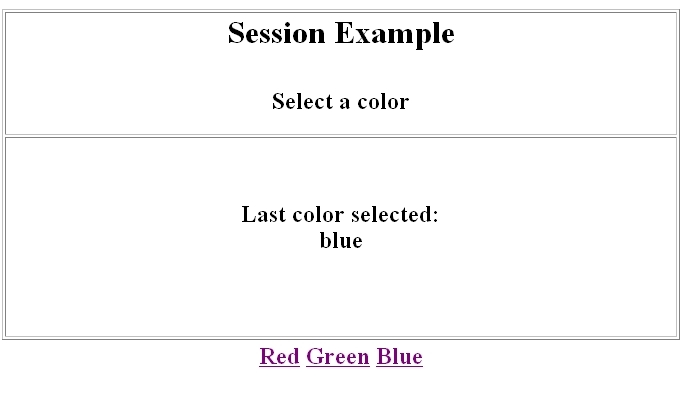
\includegraphics[clip,width=\sgw]{pics/modules/34}
\end{center}
\caption[Default template output Blue]{Default tmplate output Blue.}
\label{SessionExample}
\end{figure}

... and the template section named {\name "page2"} is activated by using the
templateSelector after clicking on a link (as you can see the color
Green was selected here) (figure~\ref{SessionExample2}).

\begin{figure}
\begin{center}
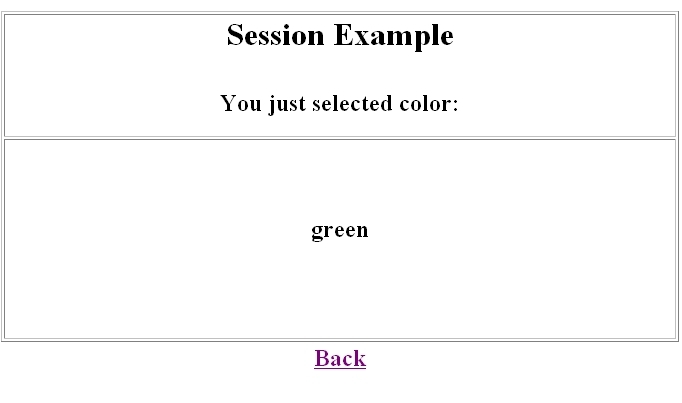
\includegraphics[clip,width=\sgw]{pics/modules/35}
\end{center}
\caption[Default template output Green]{Default template output Green.}
\label{SessionExample2}
\end{figure}

Here you can see the controlling Java method that stores the data in the
session and switches between the pages by setting the template selector.
In the session statement, a new session is created, or an existing one is
fetched. The color that was selected is attached to the HTTP request as
follows: http://www.opencms.org/sessionexample?colorvalue. To get the
query string that is attached to the HTTP link, the method
{\meth getQueryString()} is called. If a color was saved in the previous session,
it is fetched again, and displayed on the first page as the last color
that was selected. On the first page, the user is able to select one of
three colors, whilst on the second page only the "back" link can be
selected. Depending on the link with the attached query string that is
selected by the user, the template selector is set to either the first
or the second page:

\begin{java}
public byte[] getContent(CmsObject cms, String templateFile, String\\
elementName, Hashtable parameters, String templateSelector) throws CmsException \{\\
\jtabc        //init\\
\jtabc        String colorValue;\\
\jtabc        String lastColorValue="";\\
CmsXmlTemplateFile templateDocument =\\
getOwnTemplateFile(cms, templateFile, elementName, parameters,\\
templateSelector);\\
//create new or fetch existing session\\
CmsSession session = (CmsSession)\\
cms.getRequestContext().getSession(true);\\
\jtabc        //get the query string from the link\\
colorValue = ""+((HttpServletRequest)\\
cms.getRequestContext().getRequest().\\
getOriginalRequest()).getQueryString();\\
\jtabc        //get the stored value from the session\\
\jtabc        lastColorValue = (String) session.getValue("colors2");\\
\jtabc        //go back to start page\\
\jtabc        if (colorValue == "back") \{\\
\jtabd                colorValue="null";\\
\jtabd                templateSelector="default";\\
\jtabb        \}\\
\jtabb        //color chosen?\\
\jtabb        if (colorValue !="null")\{\\
\jtabd                session.putValue("colors2",colorValue);\\
\jtabd                templateSelector="page2";//show second page\\
\jtabb        \}\\
\jtabb        //inital state of the page if (colorValue.equals("null") ||\\
colorValue.equals("") ||\\
colorValue.equals("back"))\{\\
\jtabe                        olorValue="white";\\
\jtabe                        emplateSelector="default";\\
\jtabb        \}\\
\jtabb        //set process data\\
\jtabb        templateDocument.setData("bgcolor",colorValue);\\
\jtabb        templateDocument.setData("lastcolor",lastColorValue);\\
return startProcessing(cms, templateDocument,\\
elementName, parameters, templateSelector);\\
\}\\
\}\\
\end{java}

\subsection {Session content}
%============================================================================

This example dumps the keys and corresponding values that are stored in
a session. The below example displays the preceding example's session
keys and values. As you can see, the value "red" attached to the clicked
link "Red" is stored in key "colors2" of the session. The other keys and
values were generated by the system automatically for internal
use (figure~\ref{SessionExample3}).

\begin{figure}
\begin{center}
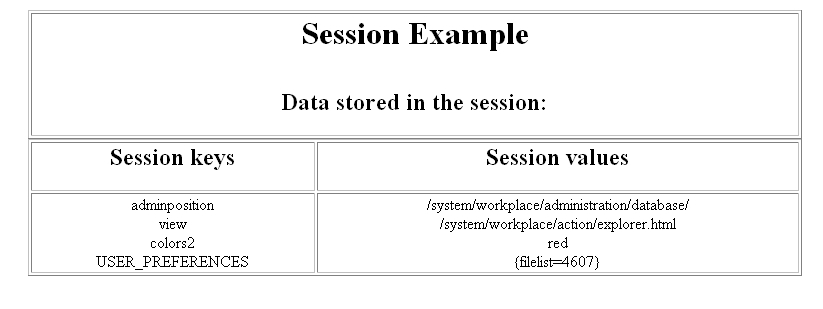
\includegraphics[clip,width=\sgw]{pics/modules/36}
\end{center}
\caption[Session Content Example]{Session Content Example.}
\label{SessionExample3}
\end{figure}

The keys of the fetched session are stored in a string array, and the
corresponding values are read out in a loop by the Java method. After
fetching the session, the session key strings are created by using the
{\meth getValueNames()} method. By looping through the entries of this string
array the corresponding values are read out by the {\meth getValues()} method.
Finally the data is set in the template document by using the {\name setData()}
method:

\begin{java}
public byte[] getContent(CmsObject cms, String templateFile,
String elementName, Hashtable parameters, String templateSelector)
throws CmsException \{\\
\jtabc        //init\\
\jtabc        String tempKey="";\\
\jtabc        String tempValue="";\\
CmsXmlTemplateFile templateDocument =\\
getOwnTemplateFile(cms, templateFile, elementName, parameters,\\
templateSelector);\\
\jtabc        //create new or fetch existing session\\
CmsSession session = (CmsSession)\\
cms.getRequestContext().getSession(true);\\
\jtabc        //copy sessionkeys into stringarray\\
String [] sessionKey = session.getValueNames();\\
\jtabc        //loop through sessionkeys\\
\jtabc        for(int i=0;i < sessionKey.length;i++) \{\\
\jtabd                tempKey += sessionKey[i]+"<br>";\\
tempValue += session.getValue(sessionKey[i])+"<br>";\\
\}\\
\jtabc        // set data in xml-document\\
\jtabc        templateDocument.setData("sessionkey", ""+tempKey);\\
templateDocument.setData("sessionvalue", ""+tempValue);\\
\jtabd                // Finally start the processing\\
\jtabc        return startProcessing(cms, templateDocument,\\
elementName, parameters, templateSelector);\\
\}\\
\end{java}

\subsection {Session history}
%============================================================================

As mentioned above, you can store any object you like in the session,
e.g. strings, arrays or vectors. The following example makes use of this
feature by storing data of the past query strings in the session. The
example shows the past five color links you clicked and deletes the
oldest one, if you clicked more than five times (figure~\ref{SessionExample4}).

\begin{figure}
\begin{center}
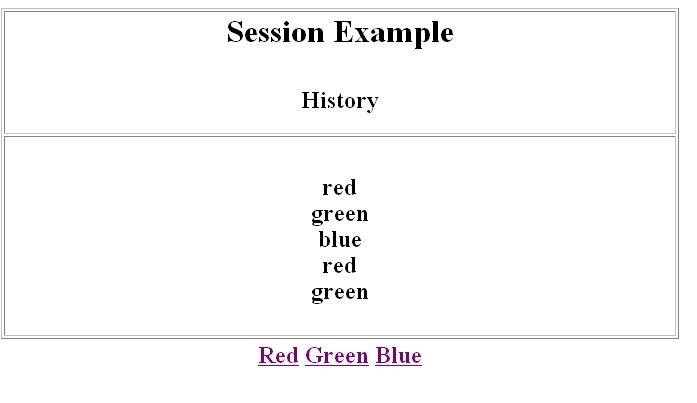
\includegraphics[clip,width=\sgw]{pics/modules/37}
\end{center}
\caption[Session history Example]{Session history Example}
\label{SessionExample4}
\end{figure}

This is done by the {\meth getContent()} method described below. The values are
stored using a string array in the session. If the array is not empty,
it is fetched from the session. The new color value that is selected by
the user is appended to the first empty entry of the array. If there is
no empty entry left in the string array, the first entry is deleted by
shifting the other entries up by one position. The new entry is moved to
the (now empty) last position. The array is stored again in the session,
and the parameters for the template are processed.

\begin{java}
\jtabc        public byte[] getContent(CmsObject cms, String templateFile,\\
\jtabc        String elementName, Hashtable parameters, String templateSelector)\\
\jtabc         throws CmsException \{\\
\jtabc        //init\\
\jtabc        String allColorValues = "";\\
\jtabc        String colorValue="";\\
\jtabc        String[] colorArray= {"","","","","","",""} ;\\
\jtabc        //set data\\
\jtabc        CmsXmlTemplateFile templateDocument =\\
\jtabc        getOwnTemplateFile(cms, templateFile, elementName, parameters,\\
\jtabc        templateSelector);\\
\jtabc        //create new or fetch existing session\\
\jtabc        CmsSession session = (CmsSession)\\
\jtabc        cms.getRequestContext().getSession(true);\\
\jtabc        //get query string from link\\
\jtabc        colorValue =\\
\jtabc        ""+((HttpServletRequest)cms.getRequestContext()\\
\jtabc        .getRequest().getOriginalRequest()).getQueryString();\\
\jtabc        // get array data from the session\\
\jtabc        if (session.getValue("colorArray") !=null)colorArray = (String [])\\
\jtabc        session.getValue("colorArray");\\
\jtabc        // fill array with data\\
\jtabc        for (int i=0;i<6;i++)\{\\
\jtabd                if (colorArray[i] == "")\{\\
\jtabe                        colorArray[i]=colorValue;\\
\jtabe                        break;\\
\jtabd                \}\\
\jtabc        \}\\
\jtabc        // if array filled shift array data\\
\jtabc        if (colorArray[5] != "") \{\\
\jtabd                for(int i=0;i<6;i++)\{\\
\jtabe                        colorArray[i]=colorArray[i+1];\\
\jtabd                \}\\
\jtabd                colorArray[5]="";\\
\jtabc        \}\\
\jtabc        for (int i=0;i<6;i++) allColorValues += "<br>"+colorArray[i];\\
\jtabc        //store data in the session session.putValue("colorArray",colorArray);\\
\jtabd                session.putValue("colors",colorValue);\\
\jtabc        //set parameters for processing\\
\jtabc        if (colorValue.equals("null") ||colorValue.equals("")) colorValue="white";\\
\jtabc        templateDocument.setData("bgcolor",colorValue)
\jtabc        ;templateDocument.setData("button",allColorValues);\\
\jtabc        return startProcessing(cms, templateDocument, elementName,
\jtabc        parameters, templateSelector);\\
\jtabc        \}\\
\}\\
\end{java}

Session management is a useful feature when building web sites
because it enables you to implement advanced features such as
HTML forms that extend over multiple pages, online shopping functionality
or personalized web content. Session management extends the abilities of
cookies that are only capable of storing text data of a limited size
(4096 Bytes) on the client. With session management, it is possible to
store binary and class information. The session management is, of course,
not only usable with query strings but also with forms. 

\section{Forms}
%============================================================================

HTML forms are used to add functionality to a website. With HTML forms,
you can receive feedback from the surfers or enable them to order
products, product-related materials, or anything else you'd like to make
available.
The input that is received from the user can be evaluated in a number of
ways. Traditionally, this is done by a cgi program that processes the
data on the server. Major drawbacks of this approach are the
inefficiency and the security holes. When using cgi programs to process
the data, every request to the cgi program creates a new process, which
produces a significant load on the server. The cgi approach
does not come with a security model that prevents incorrect cgi programs
from crashing the server.
These disadvantages have been overcome by Java servlets, which provide a
way to write efficient, platform independent, and secure
server-applications. Servlets are special Java classes that can be
executed by a server that supports the Java servlet API. Servlets take
advantage of the built in security model and the platform independence
of the Java language. An instance of a servlet is loaded either when the
server is started or when the servlet is first accessed. 
Concurrent requests to one servlet
are handled by multiple threads of the servlet. After a servlet is first
loaded and initialized, it is generally not unloaded until the server
shuts down. This ensures the servlet class is loaded and initialized
once when the servlet is accessed for the first time.
OpenCms itself is a servlet that enables the evaluation of HTML forms and
writing customized Java classes. Although not servlets themselves, these
classes have the same advantages as servlets: they are efficient,
portable, and secure!
This chapter explains how input fields, radio buttons or select buttons
are used in forms. It also discusses programming techniques that can
(and should) be used with forms, such as validating and error checking
input, as well as redisplaying input in input fields. Starting with the
simple redisplay of text that was typed in an input field, you will
learn how to use radio buttons and evaluate input data for errors
(empty fields or incorrect inputs).


\subsection {A first example using forms}
%============================================================================

In a first and simple example, you will see how a form can be used for
plain text input and to redisplay the input on a confirmation page
after submitting the form.

Because the form shouldn't be evaluated when it is requested for the
first time, a little trick can help to detect if the form is being
displayed for the first time or if it has already been filled out. A
hidden input field in the form acts as a flag that indicates if the
form has been sent or not. The value of this hidden field
is set in the Java class. When the page is first requested, the value of
the field is not defined. The Java class detects this and omits the processing
of the form's input. This is a excerpt from the template :

\begin{xml}
<FORM>...\\
\xtaba <INPUT type="hidden" name="action"\\
\xtaba value="]]><process>setaction</process><![CDATA[">\\
...</FORM>\\
\end{xml}

The Java class reads in the parameter {\name action} and if it has no value (the form has
not been sent) sets its value to the string "default" by setting the data block
{\name setaction}:

\begin{java}
...\\
String action = (String) parameters.get("action");\\
//no button pressed!\\
if (action == null || action.equals("")) \{\\
\jtaba        templateSelector="default";\\
\jtaba        template.setData("setaction","default");\\
...\\
\end{java}

Figure~\ref{simple form} shows a screenshot of the form. It consists of
two different input fields where text can be entered.

\begin{figure}
\begin{center}
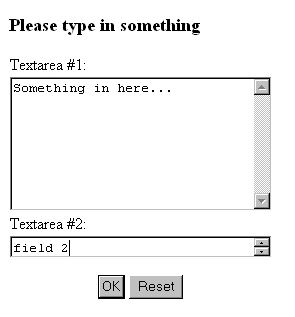
\includegraphics[clip,width=0.4\linewidth]{pics/modules/38}
\end{center}
\caption[A simple form]{A simple form}
\label{simple form}
\end{figure}

After typing in the text, you can click on the OK button to send the form, or the Reset button
to delete the input and restore the initial state of the form.
The input will be processed by a Java class and a confirmation page will be shown
which shows the text that was typed in the fields.
Figure~\ref{TypeIn} shows the message that will be presented to the user.

\begin{figure}
\begin{center}
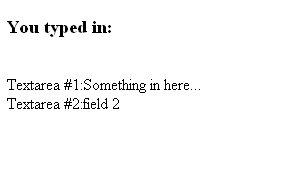
\includegraphics[clip,width=0.5\linewidth]{pics/modules/39}
\end{center}
\caption[the confirmation page]{the confirmation page}
\label{TypeIn}
\end{figure}

As you can see, the confirmation page shows the user's input again
so that the user can see what was sent to the server. The
layout and content of the confirmation page is defined in the same file
as the form inside a template with the name {\name reply}. The Java class
controls what template will be used by setting the templateselector:

{\code ...\\templateSelector="reply";\\...}

Here is the complete sourcecode of the {\meth getContent()}
method of the Java class:

\begin{java}
public byte[] getContent(CmsObject cms, String templateFile,\\
\jtabb        String elementName, Hashtable parameters,\\
\jtabb        String templateSelector) throws CmsException \{\\
\jtaba    //init\\
\jtaba        CmsXmlTemplateFile templateDocument =getOwnTemplateFile(cms,\\
\jtabc              templateFile, elementName,\\
\jtabc              parameters,templateSelector);\\
\jtaba        //button pressed?\\
\jtaba        String action = (String) parameters.get("action");\\
\jtaba        if (action == null || action.equals("")) \{\\
\jtabb              //no button pressed!\\
\jtabb              templateSelector="default";\\
\jtabb              templateDocument.setData("setaction","default");\\
\jtaba        \} else \{\\
\jtabb              //a button was pressed\\
\jtabb              //get parameters from the default template\\
\jtabb              String comment = ((String) parameters.get("comment"));\\
\jtabb              String comment2 = ((String) parameters.get("comment2"));\\
\jtabb              //set the template selector\\
\jtabb              templateSelector="reply";\\
\jtabb              //set the parameters in the reply template\\
\jtabb              templateDocument.setData("setaction","reply");\\
\jtabb              templateDocument.setData("comment",comment);\\
\jtabb              templateDocument.setData("comment2",comment2);\\
\jtaba       \}\\
\jtaba       return startProcessing(cms, templateDocument,\\
\jtabc      elementName, parameters, templateSelector);\\
\}\\
\end{java}


\subsection {Presetting values}
%============================================================================

In order to use preset values, the controlling Java class has to set the
values of the fields with a preset value or with the input the user has
already given. This can be accomplished by setting the value of a field
via the process tag:

\begin{java}
<TEXTAREA cols=30 rows=8 name=comment>\\
]]><process>comment</process><![CDATA[\\
</TEXTAREA>\\
\end{java}

The value of the input field will be the value of the data block comment.
This data block is specified in the template as an empty data block: If
you did not initialize the data block, you will get an error message
that the data block is unknown. You should always define the value  as
an empty element at beginning of the body template:

\begin{xml}
<XMLTEMPLATE>...\\
<comment></comment> ...\\
<TEMPLATE>...\\
\end{xml}

A value is preset by entering text. When the template is first started,
the data block is set with this value:

\begin{xml}
<XMLTEMPLATE>...\\
<comment>Please fill in something here!</comment>...\\
<TEMPLATE>...\\
\end{xml}

If the value is not defined in the Java class with a different value,
the data block will be empty or set to the start value, if it was
defined in the template. To show the user's input in the field, the
input first has to be fetched from the parameters that were passed to
the {\meth getContent()} method, which will set the data block comment to this
value. Below is a piece of code that shows how to do this:

\begin{xml}
String comment = (String) parameters.get("comment");\\
template.setData("comment", comment);\\
\end{xml}

The value of the field is first fetched from the parameters hash table,
which stores the parameters that are passed when the form is submitted.
The data block is then set to this value. When started for the first
time, the output of the example page with the preset comment data block
"Please fill in something here!" would look like in figure~\ref{TypeIn1}.

\begin{figure}
\begin{center}
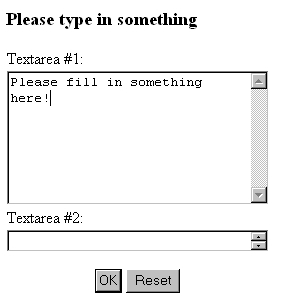
\includegraphics[clip,width=0.5\linewidth]{pics/modules/40}
\end{center}
\caption[Presetting values pic1]{Presetting values}
\label{TypeIn1}
\end{figure}


\subsection {Evaluating forms}
%============================================================================

It is desirable to evaluate input fields for empty or invalid data and
to give feedback to the user if input fields were filled out incorrectly.
Form evaluation is a typical task that is performed by a programmer.
The error checking and validation processes have to be provided by the
controlling Java class. In the following example, the user is asked to
fill out the input fields with his name, e-mail address and telephone
number. The fields marked with an * are required, the telephone number
is optional (figure~\ref{EvaluForms}).

\begin{figure}
\begin{center}
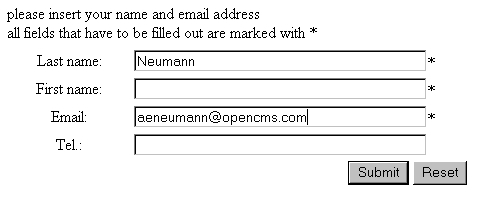
\includegraphics[clip,width=0.7\linewidth]{pics/modules/41}
\end{center}
\caption[Evaluating forms Pic 1]{Evaluating forms Pic 1.}
\label{EvaluForms}
\end{figure}

After posting the form data to the server by clicking on the OK button,
the input fields are checked by the Java class, to see if any of the
required (*) fields were left empty. The page is redisplayed with the
data that the user typed in and error messages. The user is informed
that  some of the fields were not correctly filled out. In the above
example, the user forgot to fill out the first name input field. The
following message is displayed and access to the confirmation page denied
(figure~\ref{EvaluForms1}).

\begin{figure}
\begin{center}
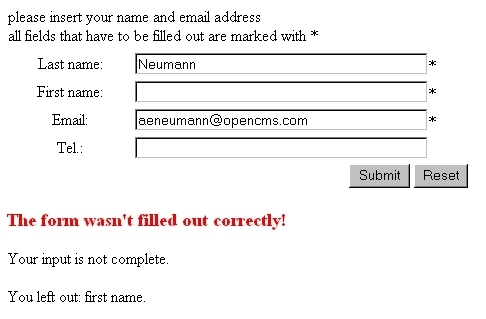
\includegraphics[clip,width=0.7\linewidth]{pics/modules/42}
\end{center}
\caption[Evaluating forms Pic 2]{Evaluating forms Pic 2.}
\label{EvaluForms1}
\end{figure}

The Java class uses preset data blocks with text phrases in the template
to display the error message in the error process at the end of the form
tag. If the input is correct, the error data block remains empty (as
initialized in the template). If there are errors (one or more of the
first three fields are empty) the page is redisplayed with the error
message using the text in the {\name init} section:
\index{error message}
\begin{java}
...\\
<!--init-->\\
<FIELD\_OMITTED><![CDATA[Your input is not complete.<br></br>\\
You left out: ]]>\\
</FIELD\_OMITTED>\\
<MISSING\_LAST\_NAME><![CDATA[last name]]></MISSING\_LAST\_NAME>\\
<MISSING\_FIRST\_NAME>\\
<![CDATA[first name]]>\\
</MISSING\_FIRST\_NAME>\\
<MISSING\_EMAIL><![CDATA[e-mail]]></MISSING\_EMAIL>\\
<GENERAL\_ERROR>\\
<![CDATA[<font color=\#FF0000><h3>The form wasn't filled out correctly!\\
</h3></font>]]>\\
</GENERAL\_ERROR>\\

<KOMMA><![CDATA[, ]]></KOMMA>\\
<POINT>.</POINT>\\
<BREAK><![CDATA[<br></br>]]></BREAK>\\
<NO\_VALUE><![CDATA[none]]></NO\_VALUE>\\

<setaction></setaction>\\
<first\_name></first\_name>\\
<last\_name></last\_name>\\
<tel></tel>\\
<email></email>\\
<error></error>\\
<!--end init-->\\
...\\
<FORM method="post">\\
...\\
<INPUT type=text maxLength=40 name=last\_name\\
value="]]><process>last\_name</process>\\
<![CDATA[" size=40>*\\
...\\
<INPUT type="hidden" name="action" value="default">\\
</FORM>\\
]]><process>{\bf error}</process><![CDATA[...\\
\end{java}


After the form data is sent, the Java code fetches the data from the
parameters hash table. It then checks the data for missing input by looking for
empty strings. If empty fields are found, an error message is generated,
and the missing data field names are concatenated with data blocks that
contain text from the template to create a more readable output of the
error message. If one field is left empty, the integer fields are
incremented and the Boolean value of the error is set to true. The
missing fields are concatenated using the data block text contained in
the template. Last but not least, the error text is returned. Below you
can see the code of the Java methods that provide the evaluation of the
input fields:

\begin{java}
private StringBuffer checkInput(Hashtable parameters,CmsXmlTemplateFile template)throws CmsException \{\\
\jtabc        boolean error = false;\\
\jtabc        boolean emailError = false;\\
\jtabc        StringBuffer errorText = new StringBuffer();\\
\jtabc        String[] missingFields = new String[3];\\
\jtabc        int fields = 0;\\
\jtabc        String lastName = ((String) parameters.get("last\_name"));\\
\jtabc        String firstName = ((String) parameters.get("first\_name"));\\
\jtabc        String email = ((String) parameters.get("email"));\\
\jtabc        String tel = ((String) parameters.get("tel"));\\
\jtabc        // check if the fields last\_name, first\_name\\
\jtabd         // and email are filled out\\
\jtabc        if {\bf(lastName.equals(""))}\\
\jtabe                missingFields[fields++] = "missing\_last\_name";\\
\jtabc        if {\bf(firstName.equals(""))}\\
\jtabe                missingFields[fields++] = "missing\_first\_name";\\
\jtabe        if {\bf(email.equals(""))} missingFields[fields++] =\\
\jtabf         "missing\_email";\\
\jtabe        // create error message when fields are omitted\\
\jtabe        if (fields > 0) \{\\
\jtabf                error = true;\\
\jtabf                errorText.append(template.getDataValue("field\_omitted"));\\
\jtabf                for (int i = 0; i < fields; i++) \{\\
\jtabf                        errorText.append(template.getDataValue(missingFields[i]));\\
\jtabf                        if (i < fields - 1) \{\\
\jtabf                        errorText.append(template.getDataValue("komma"));\\
\jtabf                        \}\\
\jtabf                \}\\
\jtabf                errorText.append(template.getDataValue("point"));\\
\jtabf                errorText.append(template.getDataValue("break"));\\
\jtabe        \}\\
\jtabe        if (error) \{\\
\jtabf        errorText.insert(0,template.getDataValue("general\_error"));\\
\jtabf                if (emailError) \{\\
\jtabe        errorText.append(template.getDataValue("email\_error"));\\
\jtabf                \}\\
\jtabe        \}\\
\jtabe        return errorText;\\
\}\\
\end{java}

The method {\meth getContent()} calls the above seen {\meth checkInput()} method, which
returns the error message. The rest of the coding is more or less the
same as seen in the previous examples:

\begin{java}
...\\
\jtabc        //no button pressed!\\
\jtabc        if (action == null || action.equals("")) \{\\
\jtabd                templateSelector="default";\\
\jtabd                template.setData("setaction","default");\\
\jtabc        //the ok button was pressed\\
\jtabc        \} else \{\\
\jtabd                String errorText="";\\
\jtabd                //check input for errors\\
\jtabd                errorText = checkInput(parameters,template).toString();\\
\jtabd                String lastName = ((String)parameters.get("last\_name"));\\
\jtabd                String firstName = ((String)parameters.get("first\_name"));\\
\jtabd                String email = ((String) parameters.get("email"));\\
\jtabd                String tel = ((String) parameters.get("tel"));\\
\jtabd                // set the fields with the given input in any case \\
\jtabd            // (even if empty String)\\
\jtabd                template.setData("last\_name", lastName);\\
\jtabd                template.setData("first\_name", firstName);\\
\jtabd                template.setData("email", email);\\
\jtabd                template.setData("tel", tel);\\
\jtabd                // if no error show reply template\\
\jtabd                if (errorText.length() == 0) \{\\
\jtabf                                templateSelector = "reply";\\
\jtabd                \} else \{\\
\jtabe                        // show default page again with error message\\
\jtabe                        templateSelector = "default";\\
\jtabe                        // set error text \\
\jtabe                        template.setData("error", ""+errorText);\\
\jtabd                \}\\
\jtabc        \}\\
\jtabc        return startProcessing(cms, template, elementName,parameters,\\
\jtabe               templateSelector);\\
\}\\
\end{java}


\subsection{Validating Forms}
%============================================================================

In order to perform a detailed check of the input data, the text must be
checked for invalid content. The above example is extended by a simple
e-mail checker. The Java method considers the e-mail address to be
valid if it contains a dot (.) and an at (@) sign. 
If this is not the case, the user sees an error message like in figure~\ref{ValidaForms}.

\begin{figure}
\begin{center}
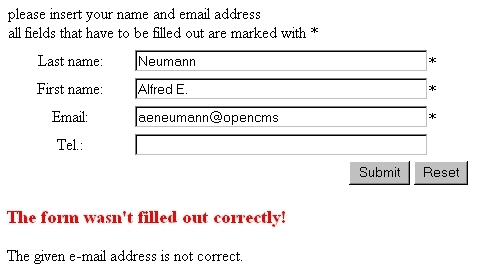
\includegraphics[clip,width=0.7\linewidth]{pics/modules/43}
\end{center}
\caption[Validating forms Pic 1]{Validating forms Pic 1.}
\label{ValidaForms}
\end{figure}

To validate the e-mail address, the Java method {\meth checkInput()} is simply
extended in the mail checking section by calling the {\meth validEmail()} method:

\begin{java}
...\\
if (email.equals("")) \{\\
\jtabc        missingFields[fields++] = "missing\_email";\\
\jtabc       \} else \{\\
\jtabc        if (!validEmail(email)) \{\\
\jtabe                error = true;\\
\jtabe                emailError = true;\\
\jtabc        \}
\}\\
...\\
\end{java}

The method {\meth validEmail()} returns true if the e-mail address is valid or false
otherwise: 

\begin{java}
\index{validEmail}
private boolean validEmail(String email) \{\\
\jtaba if (email != null \\
\jtabc        \&\& email.indexOf('.') != -1 \\
\jtabc        \&\& email.indexOf('@') != -1) \{\\
\jtabb    return true;\\
\jtaba \} else \{\\
\jtabb    return false;
\jtaba\}\\
\}\\
\end{java}


\subsection{Using radio buttons and checkboxes}
%============================================================================

HTML provides checkboxes and radio buttons for limited selections.
Radio buttons enable users to specify a selection by clicking on a field
rather than by typing in text. Checkboxes represent a group of labeled
buttons in HTML. The user is able to check none, one, or more of these
buttons that belong to the same group, which is defined by the name of
the value. The checkbox is defined in HTML as an input field tag 
of the type checkbox:

\begin{java}
<input  type=checkbox name="my\_name" value="some\_value">
\end{java}
\index{checkbox}

Radio buttons are very similar to checkboxes, except for the fact that
the user has to check exactly one button of the same group. The group is
defined by the name of the radio buttons. Clicking on another radio button
switches the old selection to the new one. The defined value is sent by
the form when the data is confirmed by clicking on the OK button. Radio
buttons are defined in HTML forms by:

\begin{java}
<input type=radio name="my\_name" value="some\_value">\\
\end{java}
\index{radio}

Figure~\ref{Feedback} is an example of a form that uses both 
radio buttons and checkboxes.
The user's selection consists of one of four radio buttons within
one group, and of three checkboxes within another group.

\begin{figure}[t]

\begin{minipage}[b]{0.49\linewidth}
\begin{center}
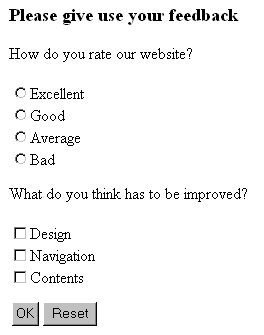
\includegraphics[clip,width=0.5\linewidth]{pics/modules/44}
\end{center}
\end{minipage}
\hfill
\begin{minipage}[b]{0.49\linewidth}
\begin{center}
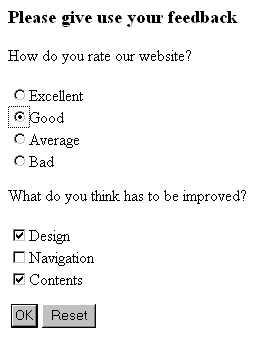
\includegraphics[clip,width=0.5\linewidth]{pics/modules/45}
\end{center}
\end{minipage}

\caption[Usage of Radio buttons]{Usage of Radio buttons}
\label{Feedback}

\end{figure}

The radio button labeled {\name Good} and the checkboxes labeled {\name Design} and {\name Contents} were
clicked by the user before the confirmation button was activated (figure~\ref{Feedback}).
The Java method {\meth checkRadio()} is used to test whether a radio button was
checked and then return the value {\name checked}. 
The Java method  is called by a method tag with two parameters:
name and value of the radio button or checkbox in the body template.
The parameters are given as a comma seperated list in the string in the {\tag <METHOD>} tag. 
The first value is the name of the radio button or checkbox 
and the second the value it has when it is checked. 
The method checks whether the radio button or checkbox was activated by getting the value
of the parameter and comparing it to the value it should have when it is selected.
If the button was activated the method returns {\name checked} or an empty String otherwise.
The string {\name checked} inside the {\tag <INPUT>} tag in HTML indicates that this radio button or 
checkbox has to be rendered as selected.
Here is an example how a checkbox is inserted in the template:

\begin{java}
...\\
<INPUT type=checkbox name=design value="design"]]>\\
<method name="checkRadio">design,design\\
</method><![CDATA[>Design\\
...\\
\end{java}

The method {\meth checkRadio()} is defined in this way:

\begin{java}
public Object checkRadio(CmsObject cms, String tagcontent,\\
\jtabb           A\_CmsXmlContent doc, Object userObject)\\
\jtabb           throws CmsException \{\\
\jtaba        Hashtable parameters = (Hashtable) userObject;\\
\jtaba        String returnValue = "";\\
\jtaba        int kommaIndex = tagcontent.indexOf(",");\\
\jtaba        if (kommaIndex > 0) \{\\
\jtabb                String radioGroup = tagcontent.substring(0,kommaIndex);\\
\jtabb                String radioName = tagcontent.substring(kommaIndex + 1);\\
\jtabb                String selected = (String) parameters.get(radioGroup);\\
\jtabb                if (selected != null \&\& selected.equals(radioName)) \{\\
\jtabc                        returnValue = "checked";\\
\jtabb                \}\\
\jtaba        \}\\
\jtaba        return returnValue;\\
\}\\
\end{java}

The {\meth getContent()} method processes the checked boxes by getting them from
the parameter's hash table and displaying the result on the confirmation
page (the template section  {\name "reply")} of the template. Predefined data
blocks in the template that contain text are used to process a readable error message.
Figure~\ref{Feedback3} shows the message that the {\meth getContent()} method produces if the input
is complete (a radio button and one or more checkboxes were checked).

\begin{figure}
\begin{center}
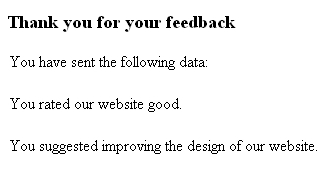
\includegraphics[clip,width=0.6\linewidth]{pics/modules/46}
\end{center}
\caption[Radio buttons Pic 3]{Radio buttons Pic 3.}
\label{Feedback3}
\end{figure}


\subsection {Presetting the values of select boxes and radio buttons in Java}
%============================================================================

As we have seen in the previous examples, presetting the values of radio
buttons is a bit tricky. The XML template mechanism tries to take care of this problem by providing
a special template class {\class com.opencms.defaults.CmsXmlFormTemplate}
that facilitates the control of select boxes and radio buttons from within the controlling
Java class. This template class allows radio buttons and select boxes to
be selected before the body template is started. If you want to create
radio buttons or select boxes with Java, your Java class has to extend
the {\class CmsXmlFormTemplate} class rather than the normally used template class
{\class com.opencms.template.CmsXmlTemplate}.

The standard HTML input tag select box that is used in the template
has to be replaced by the following method tag, which is structured in
much the same way the original HTML tag is. In its plainest form the tag
looks like this:

{\code ]]><select name="select\_1" method="my\_selectorMethod"/><![CDATA[}

The standard radio button input field is replaced by the following
method tag:

{\code ]]><radiobutton name="radio\_1" method="my\_selectorMethod" order="row"/><![CDATA[}

The main difference between the two basic tags shown above is that you
can display the radio buttons in a row or in a column layout.

The layout of the radio buttons and select boxes is defined in a special
file. Without this file, the new radio and select tags will not work.
You need to extend your workplace by the HTMLFormDefs file in the
{\dir /system/workplace/templates} directory because this file is used by the methods
{\tag handleRadiobuttonTag()} and {\tag handleSelectTag()} of the {\class CmsXmlFormTemplate}
class.

If you want to use additional statements in these tags (e.g. to change
the size) have a look at the HTMLFormDef file that can be found in your
{\dir /system/workplace/templates} directory.

Below is an example with the values "elite" for the radio button and
"other" for the select box set by the Java method (figure~\ref{RadioButtons}).

\begin{figure}
\begin{center}
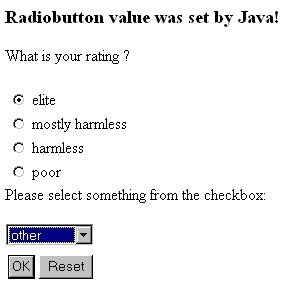
\includegraphics[clip,width=0.4\linewidth]{pics/modules/47}
\end{center}
\caption[Radio buttons in Java]{Radio buttons in Java.}
\label{RadioButtons}
\end{figure}

You can activate the radio button that should be preselected by setting
the data  in the session by a method in your Java class (normally the
{\meth getContent()} method). In this example, the Java code 

\begin{java}
{\code session.putValue("checkradio", "my\_radioname\_1")};
\end{java}

activates the radio button {\name my\_radioname\_1}.
The layout is set with {\name "order="} to rows or columns.

The template calls the method {\meth my\_radioMethod()} in the radio element.
The checked radio button that was stored in the session is displayed
with the other names and values that were added to this method.

\begin{java}
public Integer my\_radioMethod (CmsObject cms, Vector values,\\
\jtabb                  Vector names, Hashtable parameters)\\
\jtabb                  throws CmsException \{\\
\jtaba                 int index;\\
\jtaba                String checkradioValue = (String)session.getValue("radio\_1");\\
\jtaba                // add values for the checkbox\\
\jtaba                   values.addElement("my\_radiovalue\_1");\\
\jtaba                ...\\
\jtaba                // add corresponding names for the checkboxvalues\\
\jtaba                names.addElement("my\_radioname\_1");\\
\jtaba                ...\\
\jtaba                // used for the assignment of the button\\
\jtaba                   if checkradioValue.equals("my\_radiovalue\_1") index = 0;\\
\jtaba                ...\\
\jtaba                return new Integer(index);\\
                \}\\
\end{java}

To set the initial value (e.g. in the {\meth getContent()} method or even in
the {\meth my\_radio\_method()} itself), you have to create a new session (or fetch
an existing one) and store the value that is to be displayed when the
body template is first started in the session (here {\meth my\_radiovalue\_1())}:

\begin{java}
...\\     
CmsSession session = (CmsSession)\\
cms.getRequestContext().getSession(true);\\
...\\     
session.putValue("radio\_1","my\_radiovalue\_1");\\
\end{java}

You can activate the select box entry that should be initially displayed
by setting the data to activate the select box item to {\name my\_name} in
the session by a method in your Java class (normally the {\meth getContent()}
method). Your Java code should look like this:

{\code session.putValue("checkselect","my\_selectname\_1");}

The template calls the method {\meth my\_selectorMethod()} in the select element
tag. The selected select box item that was stored in the session is
displayed. The other select box names become visible after the select box
is opened.

\begin{java}
public Integer my\_selectorMethod (CmsObject cms, Vector values, Vector names, Hashtable parameters)\\
\jtabb                throws CmsException \{\\
\jtabb                int index;\\
\jtaba          String checkselectValue = (String)\\
\jtaba        session.getValue("selectbox\_1");\\
\jtaba        // add values for the selectbox\\
\jtaba        values.addElement("my\_selectvalue\_1");\\
\jtaba        ...\\
\jtaba        // add corresponding names for the selectboxvalues\\
\jtaba        names.addElement("my\_selectname\_1");\\
\jtaba        ...\\
\jtaba        // used for the assignment of the button\\
\jtaba        if checkselectValue.equals("my\_selectvalue\_1") index = 0;\\
\jtaba        ...\\
\jtaba        return new Integer(index);\\
\}\\
\end{java}

To set the initial value (e.g. in the {\meth getContent()} method or even in the
{\meth my\_selector\_method()} itself), you have to create a new session (or fetch an
existing one) and store the value that is to be displayed when the
template is first started in the session (here {\meth my\_selectvalue\_1())}:.

\begin{java}
...\\
CmsSession session = (CmsSession)\\
cms.getRequestContext().getSession(true);\\
...\\
session.putValue("selectbox\_1","my\_selectvalue\_1");\\
\end{java}
\index{session.putValue}


\subsection{Using session management with forms over multiple pages}
%============================================================================

The next example shows how you can use session management to create an
HTML feedback form that extends over multiple pages. A session provides
a way to identy a user over muliple subsequent requests and store user-related data.

Without session management, it would be impossible to
process data that was entered on the first form page in subsequent form
pages (because it would not be possible to recognize that the two requests came
from the same user). With session management, the data is stored in the session
related data area, and is therefore saved for later use.

The example consists of two subsequent HTML forms that request feedback
from the user. On the first page, the user rates the website and on the
following page he/she is asked to provide personal information such as
name and e-mail address. When all of the information has been provided,
a confirmation page will show the user's input. Because of
the session management, the data that were sent on the first page are
saved in the session and are available when the confirmation page is created.
In this example, all of the values in the session are
stored in a newly created hash table. This is the easiest way to ensure
that other values in the session are not affected by your activities. 
Imagine multiple programmers developing different HTML forms
using session management. They can easily get confused if they store
parameters with the same name in the session. It is safest to create an
extra hash table and to stores in it the session with a
(hopefully) unique name.

Below is a piece of code that shows how this is done :

\begin{java}
if (action == null || action.equals("")) \{\\
\jtaba    if (session.getValue("myForm") != null) \{\\
\jtabb        session.removeValue("myForm");\\
\jtaba    \}\\
\jtaba    session.putValue("myForm", new Hashtable());\\
\jtaba    template.setData("setaction", "page1");\\
\} else \{\\
\jtaba    if (action.equals("page1")) \{\\
\jtabb        statements...\\
\jtaba    \}\\
\}\\
\end{java}

Here you can see how the program recognizes on which page the user
currently is. The hidden HTML form input field {\name action} is used to
indicate the current page. The value of the parameter {\name action} will be an empty
string when the site is requested for the first time. In this case, the
system checks if the hash table that stores the parameters is already
contained in the session. If this is the case, it will be removed and a
new one will be created to store the new values. The value of the {\name action} parameter 
is then set to {\name page1}, and when the page is requested again
the program will check the input fields of page1.

When the fields are filled out correctly the values are stored in the
hash table:
\begin{java}
Hashtable formData = (Hashtable) session.getValue("myForm");\\
formData.put("name");\\
formData.put("email");\\
\end{java}


These values can be fetched again later using the {\meth  get()} method of the
hash table. The rest of the program is similar to the above examples
because the validation of the HTML input fields is performed in the same
way as in the previous examples.
Basically, session management allows you to store data that is related
to a special session over a period of time. In general, the session
automatically expires if it has been inactive for more than 30 minutes.


\subsection{Sending e-mails}
%============================================================================

After the forms have been processed you have all the information from
the user that you need. To determine the usability of the collected
information (e.g. for the owner of the website) it has to be forwarded to
someone for analysis. One of the easiest and most common ways of exchanging
information on the web is sending an e-mail. All you have to do to
send the collected information by e-mail, is to import a special class
and add some code to the method that will execute the mail delivery
routine. 
The XML template class used to send e-mails is the class {\class com.opencms.defaults.CmsMail} .
This class has to be included in an import statement in your template class
if you want to use it to send an e-mail.

To allow easy changes of your data input, you should store every text 
that should appear in the email in data blocks in your template. 
This enables you to change the text without the need to recompile your Java
code. 
Below is an example of such an email text data block in a template:

\begin{java}
...\\
</TEMPLATE>\\
<EMAILTEXT>\\
<![CDATA[\\
Hello ]]><PROCESS>name</PROCESS><![CDATA[,\\
This is an automatic email reply.\\
Your data:\\
Name:           ]]><PROCESS>name</PROCESS><![CDATA[\\
Surname:        ]]><PROCESS>surname</PROCESS><![CDATA[\\
email:  ]]><PROCESS>email</PROCESS><![CDATA[\\
Tel.:           ]]><PROCESS>number</PROCESS><![CDATA[\\
Date:           ]]><PROCESS>date</PROCESS><![CDATA[\\
Thank you!\\
]]>\\
</EMAILTEXT>\\
</XMLTEMPLATE>\\
\end{java}

In the {\meth getContent()} method the data blocks are fetched from the template.
If they are fetched for the first time, the data blocks are initialized as empty strings.
The data is validated after the confirmation button is
pressed (clicked on). If the validation is successful, the data is sent
to the confirmation page of the template and the whole e-mail text is
fetched as one single string by the {\meth getContent()} method. 
The e-mail text can now be sent as the e-mail content:

\begin{java}
...\\
//read the content (blank at the first start)\\
String vorname=(String)parameters.get("surname");\\
String name=(String)parameters.get("name");\\
...\\
// check if the form is displayed for the first time.\\
//If so, preset all input fields with blanks\\
if ((action==null) || (action.length()<1))\{\\
template.setData("surname","");\\
template.setData("name","");...\\
\} else \{...\\
// the form is not called the first time,\\
// analyze the given data\\
...\\
//data was validated, set data in body template\\
template.setData("name", name);\\
String mailText = template.getProcessedDataValue("EMAILTEXT");\\
...\\
//send mail and start the processing\\
\end{java}

It is important to validate the collected values {\bf before} you send the
e-mail. To send the e-mail in Java, a code fragment like the following
has to be added to your {\meth getContent()} method:

\begin{java}
...\\
//send mail and start the processing\\
//the recipient(s) of the mail\\
String receiver [] = \{"receiver\_1@somewhere.com", "receiver\_2..."\};\\
CmsMail mail =\\
new CmsMail(cms, sender, receiver, subject, content, "text/plain");\\
mail.start(); //start thread to send the mail\\
...\\\end{java}


The variables passed to the constructor of the {\class CmsMail} class are:

\begin{itemize}
\item[-] cms (type {\code org.opencms.file.CmsObject}) object to access system resources.
\item[-] sender (type {\code java.lang.String}) the e-mail address of the mail sender.
\item[-] receiver (type {\code java.lang.String[]}) one or more e-mail addresses of e-mail recipients.
\item[-] subject (type {\code java.lang.String}) the subject of the e-mail.
\item[-] content (type {\code java.lang.String}) the body (content) of the e-mail.
\item[-] type (type {\code java.lang.String}) the mime-type of the e-mail content.
The mime-type is usually set to "text/plain" for pure text mails.
\end{itemize}

Note that there are other constructors of the class {\class CmsMail} that allow to send e-mail
to cc and bcc recipients. Just have a look at the class if you need this functionality.

You can attach additional files to the mail by using the method:

\index{addAttachement}
{\meth  addAttachement(String content,String type)} 

{\bf Note:} The sending of the e-mail runs as a seperate thread. This means the program is not
blocked, even if the mail can not be sent right away!

The mail server used to send the mails can be configured in the registry of OpenCms.
The registry resides in the file {\name registry.xml} in the folder {\dir WEB-INF/config}
of your webapplication.

Here is the part of the {\name registry.xml} file where the mail server is configured:

\begin{xml}
<smtpserver>my.smtp.server</smtpserver>
<smtpserver2>alternative.smtp.server</smtpserver2>
<defaultmailsender>nobody@nowhere.com</defaultmailsender>
\end{xml}

The tag {\code <smtpserver>} contains the server that will be used first.
If this server cannot be accessed the system tries to use the server given in the tag
{\code <smtpserver2>}.
The {\code <defaultmailsender>} is used for the e-mail address of the sender
if no sender was given when creating the e-mail.


\subsection {Personalization}
%============================================================================

XML templates enable the creation of personalized web content and
the management of users and their profiles. With OpenCms' built in user
management, you can store user-related data and use advanced features
such as the management of different groups of users.
Web page content is easily adapted to each user's profile and
preferences. In order to provide personalized web content, the user's
data and preferences must be known by the system. A user that wants to
take advantage of personalized web content first has to register. He/she
can either specify their preferences manually or let them be
automatically generated by enabling the system to analyze their surfing habits.
The next example shows how a user is identified by means of a simple
login box and how the user data is extracted from the system. The
example program presents a login screen to the user. After the user
has successfully logged in, his/her personal data such as name and
address are displayed on the screen.
To test the example, you have to enter the name and password of an
existing OpenCms user. You can either create a new user for the purpose
of a test, or use the one that you use to access the system. When you
test the example, be aware that you will be working on the system under
the user account that you logged in under. You have to log in again in
order to work under your old account.
The login screen is a simple HTML form with two text input fields 
(figure~\ref{Password}). 
The login is performed by the method {\meth login()} of the class 
{\class CmsObject}. The method has the following structure:

{\code public String login(String username, String password)\\
throws CmsException;}

\begin{figure}
\begin{center}
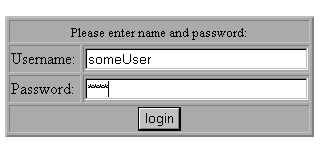
\includegraphics[clip,width=0.4\linewidth]{pics/modules/48}
\end{center}
\caption[Personalization Pic 1 ]{Personalization Pic 1.}
\label{Password}
\end{figure}

The method returns the login name when the login was successful,
otherwise it throws a {\class org.opencms.main.CmsException}. 
The exception can be captured and an appropriate error message 
showed to the user.

\begin{figure}
\begin{center}
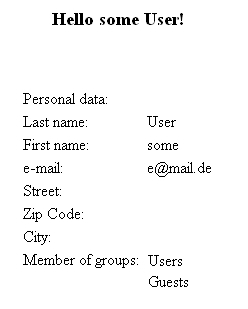
\includegraphics[clip,width=0.4\linewidth]{pics/modules/49}
\end{center}
\caption[Personalization Pic 2]{Personalization Pic 2.}
\label{HelloUser}
\end{figure}

\begin{java}
...\\
try \{\\
\jtabc                cms.loginUser(name, pass);\\
\jtabc                ...\\
\jtabc                templateSelector = "logged\_in";\\
\jtaba          \} catch (Exception e) \{\\
\jtabc                e.printStackTrace(System.err);\\
\jtabc                template.setData("setaction", "send");\\
\jtabc                templateSelector = "error";\\
\jtaba        \}\\
...\\
\end{java}

The user data is accessed via the methods of the {\class org.opencms.file.CmsUser} class. 
Several get methods can be used to fetch user data such as the first and last
name and the e-mail address. A hash table is used to store additional
information, which is defined and passed using the methods:

\begin{java}
public setAdditionalInfo(String key, Object obj);\\
public Object getAdditionalInfo(String key);\\
\end{java}

Figure~\ref{HelloUser} shows the output for the above logged in example user.

In addition to the name and e-mail address, additional information
fields can be used to capture use-related data that is essential to
create personalized content.

An alternative to using the additional information hash table would be
to customize OpenCms' user management. Since OpenCms is an open source
project you are free to modify the user management by inheriting the
existing classes or extending the existing ones with additional features.